\documentclass[english,11pt]{article}
\usepackage[utf8]{inputenc} 
\usepackage[T1]{fontenc}
\usepackage{mathpazo,amsmath,amssymb,subcaption,graphicx,amsthm,tikz-cd,graphicx}
\usepackage{amsthm, tikz-cd}
\usepackage[backend=bibtex,style=numeric-comp,natbib=true]{biblatex} 
\usepackage{relsize}
\usepackage{xcolor}
\addbibresource{references.bib}

\usepackage{geometry}
\geometry{letterpaper}

\usepackage{systeme}

\title{Volume of Simplicial Complex Polytopes}
\author{Eliana Tolosa and Jerónimo Valencia}
\date{December 2020}

\newtheorem{theorem}{Theorem}[section]
\newtheorem{corollary}{Corollary}[theorem]
\newtheorem{lemma}[theorem]{Lemma}
\theoremstyle{definition}
\newtheorem{definition}{Definition}[section]
\theoremstyle{definition}
\newtheorem{proposition}{Proposition}[section]
\theoremstyle{definition}
\newtheorem{example}{Example}[section]
\theoremstyle{remark}
\newtheorem*{remark}{Remark}
\theoremstyle{definition}
\newtheorem{question}{Question}[section]

%Configurar el paquete de presentación de código
\usepackage{listings}
\definecolor{codegreen}{rgb}{0,0.6,0}
\definecolor{codegray}{rgb}{0.5,0.5,0.5}
\definecolor{cblue}{rgb}{0.15,0.15,1.00}
\definecolor{codepurple}{rgb}{0.63,0.13,0.94}
\lstdefinestyle{mystyle}{
    commentstyle=\color{codegreen},
    keywordstyle=\color{blue},
    numberstyle=\color{codegray},
    stringstyle=\color{codepurple},
    basicstyle=\ttfamily,
    breakatwhitespace=false,         
    breaklines=true,                 
    captionpos=b,                    
    keepspaces=true,                 
    numbersep=5pt,                  
    showspaces=false,                
    showstringspaces=false,
    showtabs=false,                  
    tabsize=2
}
\lstset{style=mystyle}

\begin{document}

\maketitle

\section{Introduction}

It is well known that calculating volumes of polytopes is not an easy task. Even for three dimensional polytopes, for which we can have a visual idea, very few formulas have been derived. Therefore, the search for a satisfying formula to calculate volumes of general polytopes is still ongoing. It is common to reduce the problem to a smaller set of objects for which it is possible to find the wanted answer. This method has given some formulas for the volume of some families of polytopes. We now know that the volume of the regular permutahedron $P_n(n, n-1,\dots, 1)$ is $n^{n-2}$. This number has a nice combinatorial interpretation: it is the number of trees on $n$ labelled vertices. In \cite{Postnikov-PAB}, Alexander Postnikov, introduced a formula to calculate the volume of \textit{generalized permutahedra}, that are polytopes obtained from usual permutahedra by parallel traslations of their faces. Postnikov derives his formula by representing such permutahedra as weighted Minkowski sums of the coordinate simplices, that is $\sum y_I \Delta_I$. The class of \textit{generalized permutahedra} includes interesting families of polytopes such as associahedra, cyclohedra, graph associahedra, Pitman-Stanley polytopes, graphical zonotopes among others. Hence, finding a formula for the volume of generalized permutahedra, means being able to calculate the volume for all such families.

Nonetheless, the formula derived by Postnikov has a downside. Calculating the volume requires to find certain collections of subsets of $[n]$. Finding these collections is a high complexity problem and there does not seem to exist a nice interpretation of these collections. Therefore, it might be beneficial to restrict the family of generalized permutahedra to a smaller family in which there is a less complex formula or a nicer interpretation of the mentioned collections.
In this paper we will show our approach towards understanding and interpreting the formula for the volume of generalyzed permutahedra. We describe a method for understanding the $J-sets$ required in the formula and we summarize it in what we called $C-$\textbf{Tangram game}. We implemented an algorithm that describes the strategy for the \textit{"game"} using Python, and we obtained the same results given by an implemented method in Sage. We also computed the volumes for some polytopes related to certain families of simplicial complexes using computational implementation, in order to find a satisfactory formula for such volumes. Unfortunately, we could not derive any conclusions as calculating the volume is computationally expensive and we could not get enough data.

\subsection{Graphical zonotopes}

Given a graph $G$ with $n$ vertices, we can associate a zonotope $Z_G$ in $\mathbb{R}^n$ given by the Minkowski sum of segments indexed by the edges of such graph. Explicitly, $$Z_G = \sum_{\{ij\}\in\text{E}(G)}\left[\vec{e}_i,\vec{e}_j\right] = \sum_{\{ij\}\in\text{E}(G)}\left[0,\vec{e}_i-\vec{e}_j\right]$$
where $\left\{\vec{e}_i \ | \ 1\leq i\leq n \right\}$ is the canonical basis for $\mathbb{R}^n$. 

\begin{example}
Consider the complete graph in 3 vertices $K_3$. Then, labelling the vertices $1, 2$ and $3$ we have $Z_{K_3} = \left[\vec{e}_1,\vec{e}_2\right]+\left[\vec{e}_1,\vec{e}_3\right]+\left[\vec{e}_2,\vec{e}_3\right]$ which is the standard permutahedron $P_3$. In general, taking the graphical zonotope associated with the complete graph in $n$ vertices gives the standard permutahedron $P_n$. 
\end{example}

For these polytopes the following proposition describes a combinatorial formula for computing its volume. This proposition will be proven in two different ways. The one presented in this section relies in the general theory of zonotopes and a particular kind of subdivision used to study their Ehrhart theory \cite{beck2008computing}. In the next section we give a proof using Berentein-Kushnirenko's theorem \cite{Ber-Kush}. 

\begin{proposition}
For a connected graph $G$ on $n$ vertices, the volume of $Z_G$ equals the number of spanning trees of $G$. 
\end{proposition}

\begin{proof}
Consider the following subdivision of a zonotope in $\mathbb{R}^n$: if the polytope is given by $Z = Z(\vec{v}_1,\ldots,\vec{v}_k) = \{ \sum \lambda_i \vec{v}_i \mid 0 \leq \lambda_i \leq 1\}$ then it can be written as a union of smaller zonotopes $Z(\vec{i_1},\ldots,\vec{i_n})$ where the set $\{\vec{v}_{i_j}\}$ is a basis for $\mathbb{R}^n$. Adapting the proof of Lemma 9.1 in \cite{beck2008computing}, this is actually a subdivision of the polytope $Z$. In the graphical case, each of the smaller zonotopes which compose the subdivision have the same volume. Normalizing the volume such that each piece has volume $1$, it remain to count the number of such parts. That is, counting the number of basis of $\mathbb{R}^n$ which can be formed from the set $\{ \vec{e}_i - \vec{e}_j \mid ij\in E(G)\}$. Note that a subset of these vectors is linearly dependent if and only if the corresponding edges form a circuit in the graph. Thus, basis correspond to maximal sets of edges which do not form any circuit. That is, generating trees of the graph.
\end{proof}

\begin{example}
Taking $G=K_3$, the subdivision used in the above proposition is shown in Figure \ref{fig:zon-sub-K3}. Denoting $\vec{e}_{ij} = \vec{e}_i-\vec{e}_j$, the basis appearing are $\{\vec{e}_{12},\vec{e}_{13}\}$, $\{\vec{e}_{12},\vec{e}_{23}\}$ and $\{\vec{e}_{13},\vec{e}_{23}\}$. Therefore, $\text{vol}(Z_{K_3}) = 3$. However, this calculation assumes the volume of each parallelogram is 1. However, using the normalized volume, that is, the volume of a simplex equal to 1, those zonotopes have volume 2. This is going to be the convention throughout the document. 

\begin{figure}[!]
    \centering
    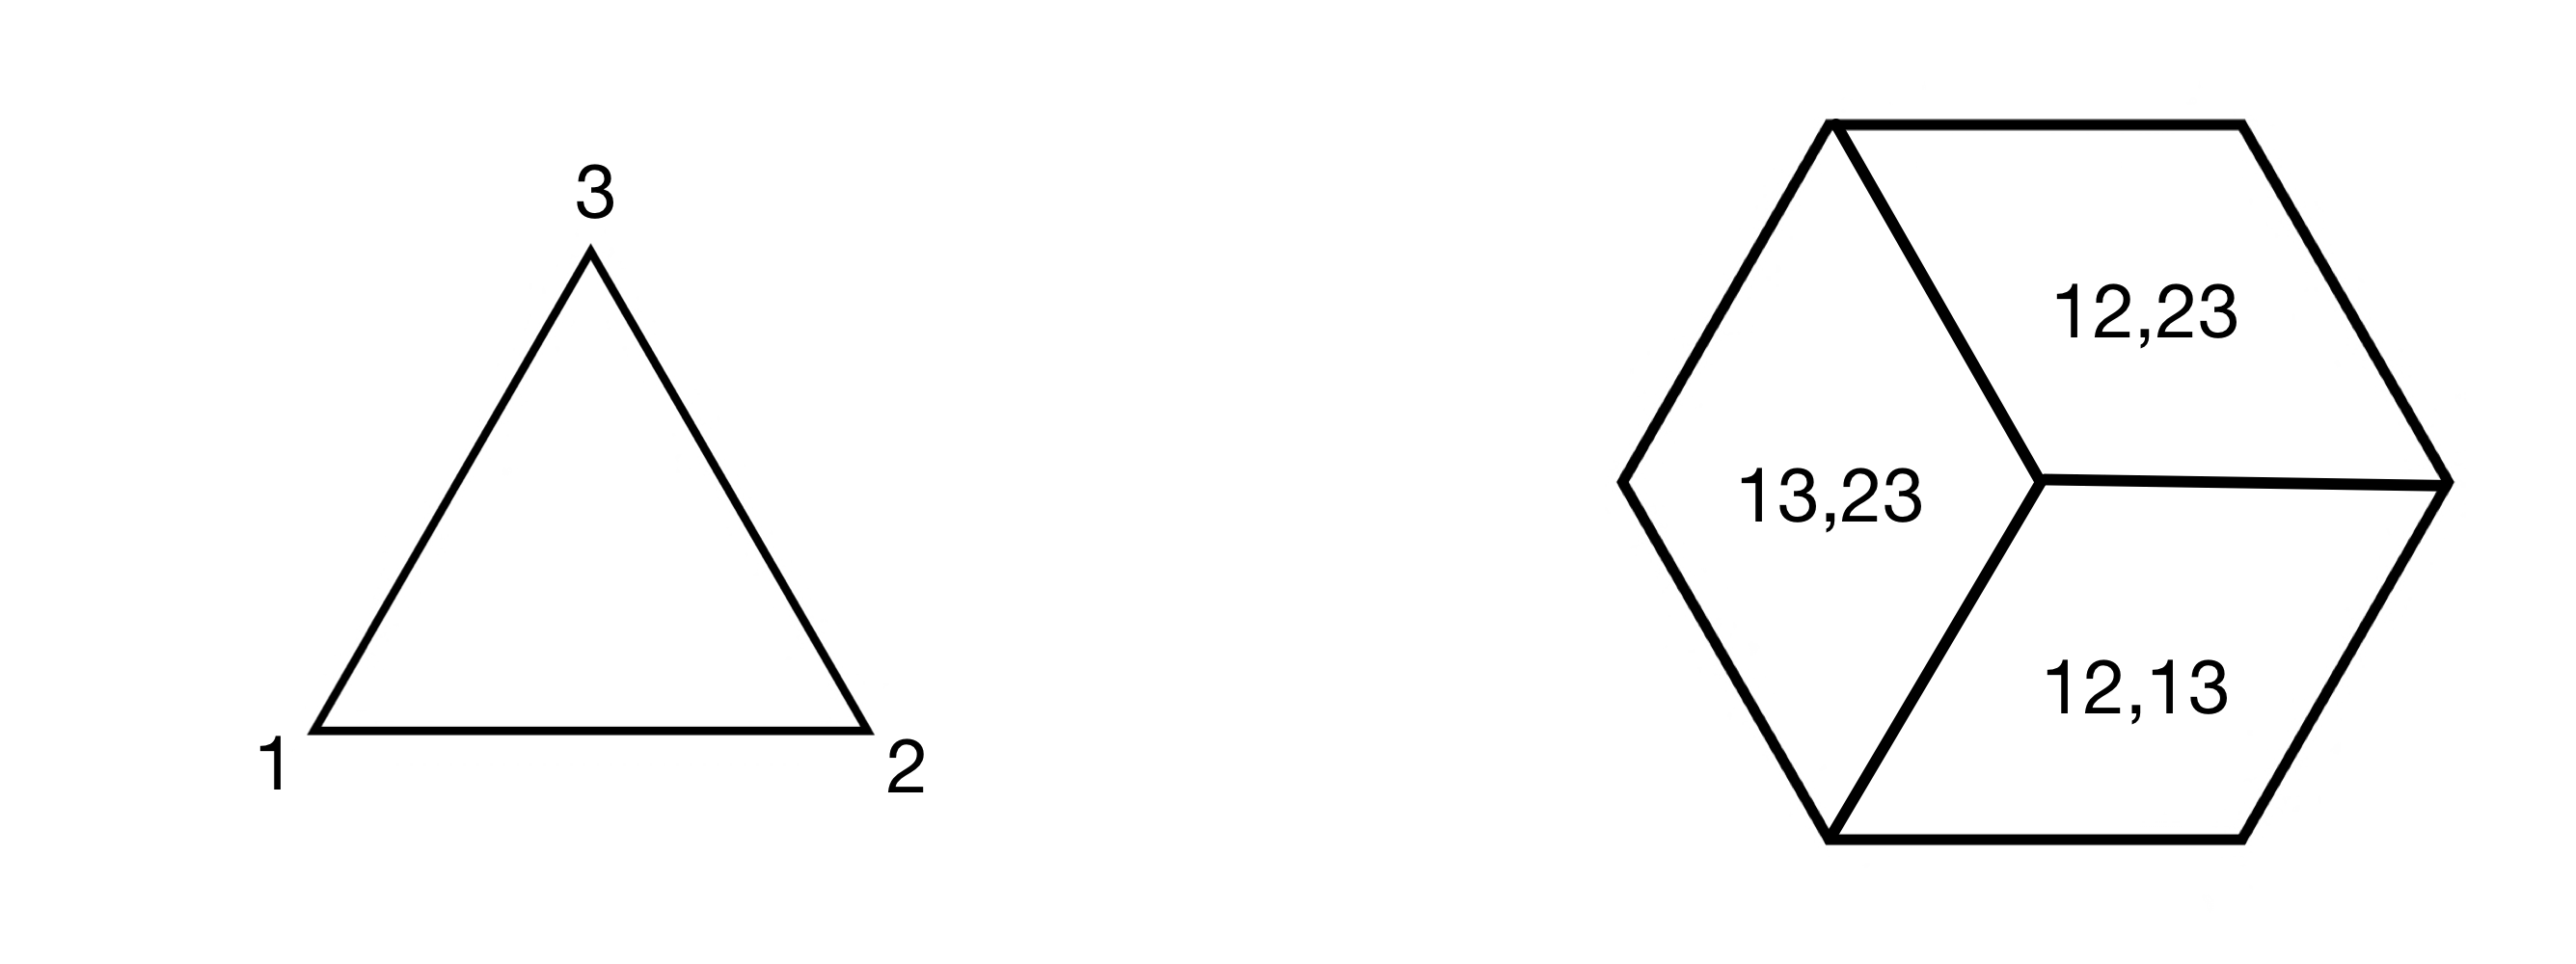
\includegraphics[scale=0.12]{images/ZonSubK3.png}
    \caption{Labeling for the graph and zonotopal subdivision of $P_{K_3}$. }
    \label{fig:zon-sub-K3}
\end{figure}
\end{example}

\subsection{Simplicial complex polytopes}

We generalize the definition of graphical zonotopes so simplicial complexes. However, in this case, the resulting polytope is not necessarily a zonotope. Therefore, computing the volume is not straightforward as in the previous case. 

By a \textbf{simplicial complex} we refer to a collection of subsets $I\subset [n]$ which label the vertices of simplices in a polytopal complex. Graphically, this accounts to taking simplices of multiple dimensions and putting them together such that each intersection is also a simplex. Now, given a simplicial complex $C$, we define the \textbf{simplicial complex polytope} $P_C$ as the Minkowski sum of the simplices comprising the complex. That is, if $C = \{ I_1,\ldots,I_n\}$ then $P_C = \sum_{i=1}^n \Delta_{I_i}$ where $\Delta_I := \text{conv}\{ \Vec{e}_i \, \mid \, i\in I \}$. 

\begin{example}
Continuing with the previous example, consider the simplicial complex $C_3 = 2^{[3]}$. For the calculation of $P_{C_3}$ we avoid the singletons as they only contribute with a parallel translation of the polytope. Figure \ref{fig:P_C_3} shows the polytope obtained. Note that the graphical zonotope $Z_{C_3^{(1)}}$ of the 1-skeleton of the complex is a subpolytope of $P_{C_3}$, as the figure shows. 

\begin{figure}
    \centering
    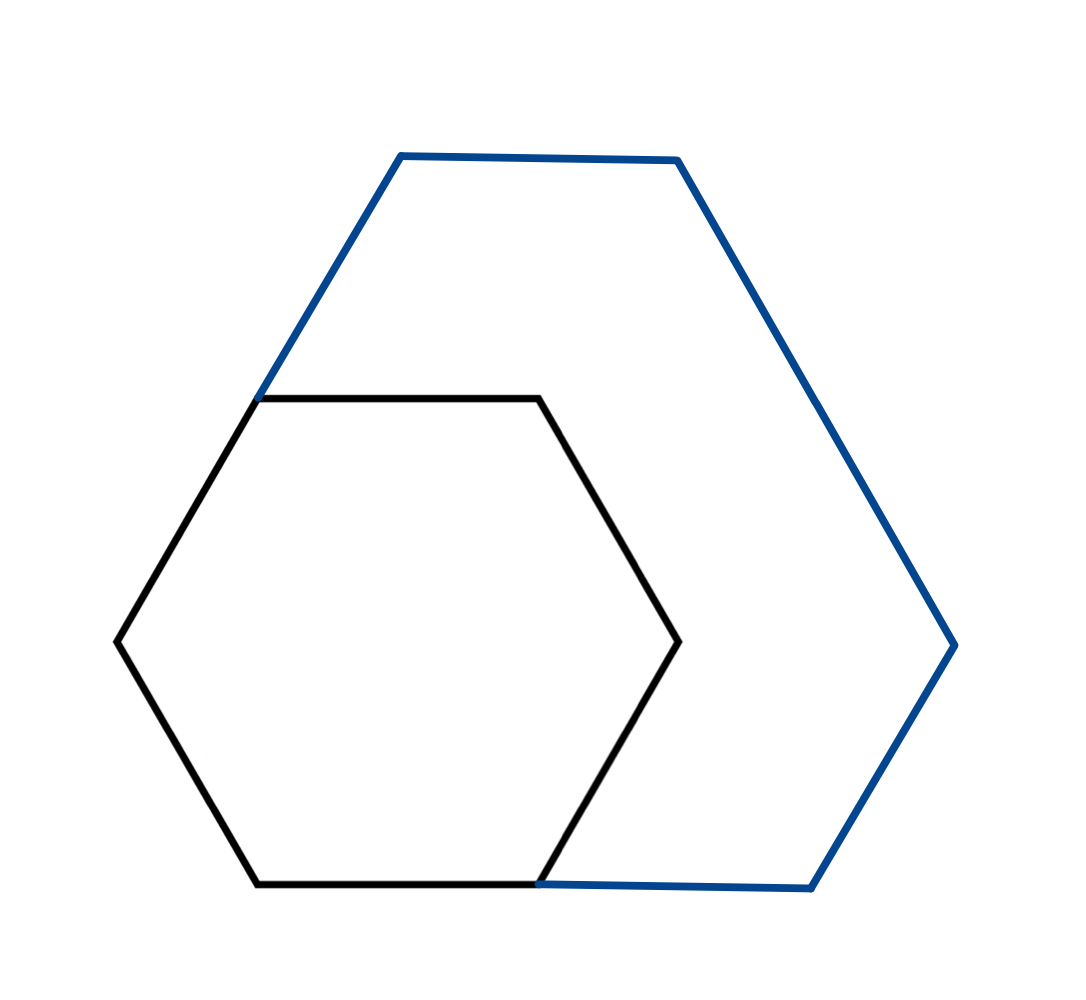
\includegraphics[scale=0.14]{images/P_C_3.png}
    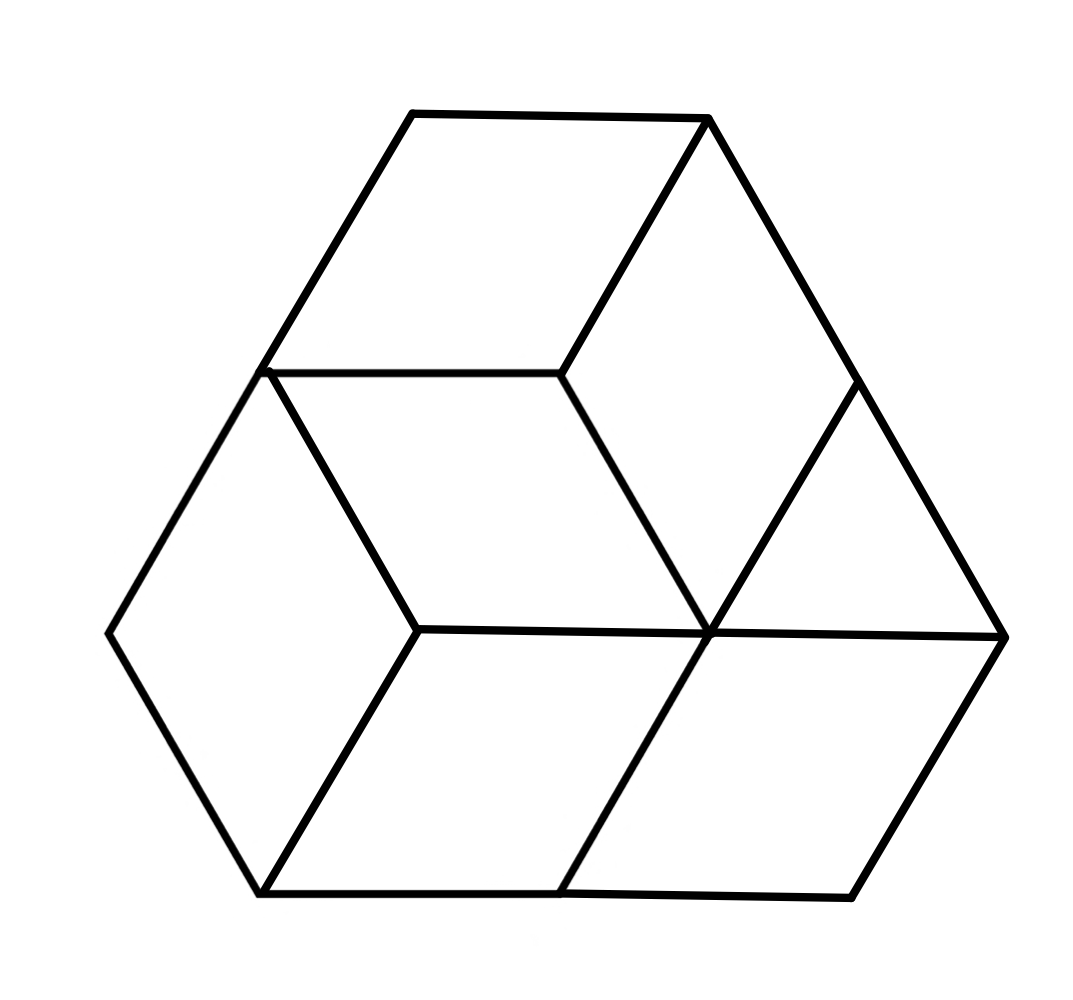
\includegraphics[scale=0.14]{images/P_C_3-subdivision.png}
    \caption{Polytope associated to the complete complex in three vertices and a particular subdivision.}
    \label{fig:P_C_3}
\end{figure}
\end{example}

As the graphical zonotope can be subdivided using zonotopes only depending on the combinatorics of the 1-skeleton of the complex, we could try to subdivide the new part added with this same pieces. However, as the figure shows, some new parts show up, and therefore the need to skip the convention on parallelograms' volume and stick to normalized volumes.\\

The question we address in this document is the following:

\begin{question}
\textbf{Given a simplicial complex $C$, how can we compute $\text{vol}(P_C)$ in a combinatorial fashion? }
\end{question}

As a first approach, let us continue with the example. The labelling of the subdivision shown in Figure \ref{fig:P_C_3-sub-marked} is similar to the one obtained when considering spanning trees of the graph. This statement will be formalized in the following section. 

\begin{figure}[!]
    \centering
    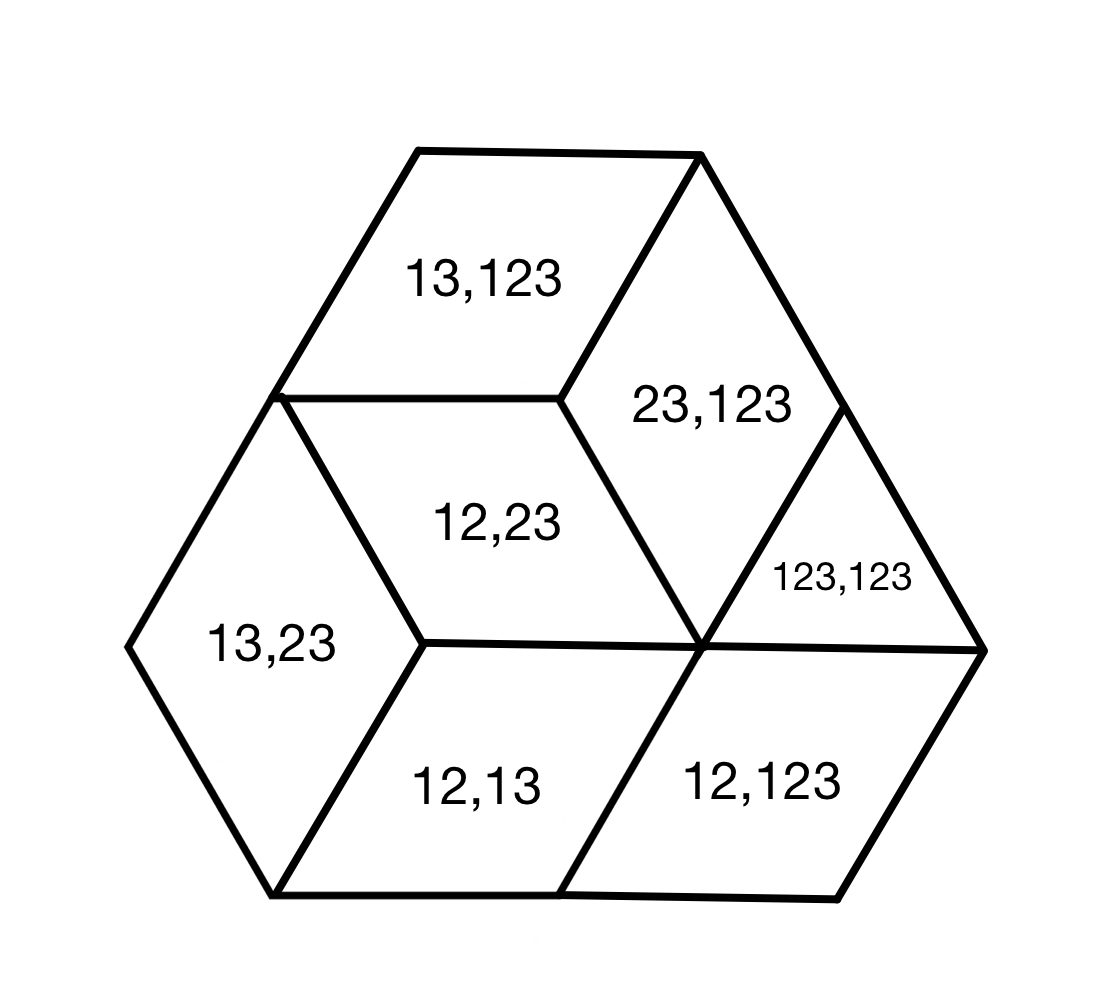
\includegraphics[scale=0.16]{images/P_C_3-subdivision-marked.png}
    \caption{Labelling of the parts of the subdivision of $P_{C_3}$.}
    \label{fig:P_C_3-sub-marked}
\end{figure}

As there is no clear path to follow in order to answer to the main question, the description of $P_C$ for any simplicial complex $C$ is exactly a description of a particular kind of generalized permutahedra. Then, using Postnikov and Lam results on this class of polytopes, some insight on the question can be given. 

\section{Generalized Permutahedra}

For this review of results on generalized permutahedra, we follow the notation in \cite{Postnikov-PAB}. A \textbf{generalized permutahedron} is a polytope obtained from the standard permutahedron by a translate of its facets which preserves the directions of its edges. In terms of its vertices, a generalized permutaedron is a convex hull of $n!$ points $\Vec{v}_w \in  \mathbb{R}^n$ labelled by permutations $w\in S_n$ satisfying $\Vec{v}_{w}-\Vec{v}_{w\cdot s_i} = \alpha_{w,i}\left( \Vec{e}_{w(i+1)}- \Vec{e}_{w(i)} \right)$ for any transposition $s_i = (i \quad i+1)$ and for some non-negative real numbers $\alpha_{w,i}$. The H-representation of a generalized permutahedron can be completely determined by a set of numbers $\{z_I\}_{I\subset [n]}$ satisfying a \textit{submodularity condition} $z_I + z_J \leq z_{I\cup J} + z_{I \cap J}$ \cite{Aguiar2017HopfPermutahedra} as follows:

$$P_z^n(\{z_I\}) = \left\{ \Vec{x}\in\mathbb{R}^n \, \mid \, \sum_{i\in[n]}x_i = z_{[n]} \text{ , } \sum_{i\in I}x_i \geq z_I \text{ for proper subsets }I\subset [n]\right\}$$
For any $I\subseteq [n]$ fix a non-negative real number $y_I$. With this data, define the polytope $$P_y^n(\{y_I\}) = \sum_{I\subseteq [n]}y_I\Delta_I$$ These polytopes are generalized permutahedra as the following propositions shows. 


\begin{proposition}
Let $\{ y_I\}$ a collection of non-negative real numbers indexed by subsets $I \subseteq [n]$ and define the numbers $\{z_I\}$ by $z_I = \sum_{J\subseteq I}y_J$. Then $P_z^n(\{z_I\}) = P_y^n(\{y_I\})$.

\begin{proof}
First, fix $I_0 \subseteq [n]$ and define $y_I = \delta_{I,I_0}$, that is $y_I = 1$ if $I=I_0$ and $y_I = 0$ otherwise. We can assume $I_0$ is not a singleton. Then $P_y^n(\{y_I\}) = \Delta_{I_0}$. In this case, $\hat z_I = 1$ if $I\supseteq I_0$ and $\hat z_I=0$ otherwise and the polytope $P_z^n(\{\hat z_I\})$ has the same inequalities defining the former simplex. Indeed, it can be directly seen that the simplex satisfies the inequalities from the definition. Now, if $\Vec{x}\in P_z^n(\{\hat z_I\})$ then $x_i \geq 0$, $\sum_{j\in J}x_j \geq 1$ for $J\supseteq I_0$ and $\sum_{j\in J}x_j \geq 0$ for $J\not\supseteq I_0$. As $\sum_{j\in [n]}x_j =1$, then $\sum_{j\not\in I_0} x_j \leq 0$ implies this is actually an equality and as all numbers are positive, this implies $x_i=0$ if $i\not\in I_0$. The remaining inequalities describe a simplex in the subspace $\text{span}\{\Vec{e}_i  \mid i\in I_0\}$ which is exactly $\Delta_{I_0}$. 

To prove the proposition, note that for any non-negative real number $\alpha$, $\alpha P_z^n(\{z_I\}) = P_z^n(\{\alpha z_I\})$ and $P_z^n(\{z_I\}) + P_z^n(\{z'_I\}) = P_z^n(\{z_I+z'_I\})$.This follows directly from the definition. Now, 

\begin{align*}
    P_y^n(\{y_I\}) &= \sum_{I\subseteq [n]}y_I\Delta_I = \sum_{I\subseteq [n]}y_I P_y^n(\{\delta_{J,I}\}) =\sum_{I\subseteq [n]}y_I P_z^n(\{\hat z_I\}) = \sum_{I\subseteq [n]} P_z^n(\{y_I \hat z_I\}) \\ 
    &= P_z^n\left(\left\{\sum_{I\subseteq [n]} y_I \hat z_I\right\}\right) = P_z^n\left(\left\{\sum_{J\subseteq I} y_I\right\}\right) = P_z^n(\{z_I\}) \\
\end{align*}
\end{proof}
\label{prop2.1}
\end{proposition}

\section{A formula for the volume of generalized permutahedra}
In this section we will show a formula for the generalizad permutahedra given by Postnikov \cite{Postnikov-PAB}. 

Consider the permutahedron $P_n(x_1,\dots, x_n)$. We can use the coordinates $y_1, \dots, y_n$ related to $x_1,\dots, x_n$ by the next equations

    \begin{align*}
        y_1 &= -x_1\\
        y_2 &= -x_2+x_1\\
        y_3 &= -x_3+2x_2-x_1\\
        & \vdots\\
        y_n&= -\binom{n-1}{0}x_n + \binom{n-1}{1}x_{n-1}\dots+ \binom{n-1}{n-1}x_1
    \end{align*}
to define the formula for the volume $V_n= \text{Vol} P_n(x_1,\dots,x_n)$ as a polynomial in the variables $y_1,\dots, y_n$.


\begin{theorem}
The volume of the permutahedron is given by 
$$\text{Vol}( P_n )= \frac{1}{(n-1)!} \sum_{(J_1, \dots, J_{n-1})} y_{|J_1|}, \dots, y_{|J_{n-1}|},$$
where the sum is given over ordered collections of subsets $J_1, \dots, J_{n-1} \in [n]$ such that, for any distinct indices $i_1, \dots, i_k$ of the $J$'s, we have $|J_{i_1}\cup \ldots \cup J_{i_k}| \geq k+1$.
\end{theorem}

Even if this is an explicit formula for finding the volume, understanding and finding the collections of $J$'s is quite tricky.

We will illustrate this with two examples, when $n=2$ and $n=3$.

\begin{example}
\begin{itemize}
    \item $n=2$: We should figure out the collection of subsets of $[n]$ that count for out sum. First notice that we will need $n-1$ subsets of $[2]$, which is only one set $J_1$. Let us take $k=1$, then $|J_1|\geq k+1= 2$. Therefore, $J_1$ should have size two and then $J_1= \{1,2\}$. Now we can conclude, that
    $$V_2= \text{Vol}(P_2)= y_{|J_1|}=y_2= x_1-x_2$$
    
    \item $n=3$: We now have to find a collection of $2$ subsets of $[3]$ that fulfill the condition. From taking $k=1$ we conclude that we should consider only the subsets with two or more elements. Let us name those sets as : $J_1=\{1,2\}, J_2=\{1,3\}, J_3=\{2,3\}, J_4=\{1,2,3\}$. From $k=2$, we conclude that we should take two subsets of $[3]$ such that their union has 3 or more elements. As $n=3$ we should consider collections of two subsets such that their union is the whole $[3]$. Those collections are: $(J_1, J_2)$, $(J_2, J_1)$, $(J_1, J_3)$, $(J_3, J_1)$, $(J_2, J_3)$, $(J_3, J_2)$, $(J_1, J_4)$, $(J_4, J_1)$, $(J_2, J_4)$, $(J_4, J_2)$, $(J_3, J_4)$, $(J_4, J_3)$, $(J_4, J_4)$. Notice that for each of the choices of possibles collections of subsets we have to consider the different orderings of them. Then we can now apply the formula and:
    \begin{align*}
        2V_3&= \text{Vol}(P_3)\\
        &= y_{|J_1|}y_{|J_2|} + y_{|J_2|}y_{|J_1|}+y_{|J_1|}y_{|J_3|}+ \dots + y_{|J_4|}y_{|J_3|} +y_{|J_4|}y_{|\hat{J}_4|}+ y_{|\hat{J}_4|}y_{|J_4|}\\
        &= 6 y_2^2 + 6y_2y_3 + y_3^2\\
        &= x_1^2+2x_1x_2-4x_1x_3-2x_2^2+2x_2x_3+x_3^2
    \end{align*}

\end{itemize}

\end{example}

An equivalent way of describing the sub-collections $(J_1, \dots, J_n-1)$ is the next condition.

\textbf{Dragon Marriage Condition}
Imagine that in a medieval town there are $n$ brides, $n-1$ grooms and a dragon. We know all the possible pairs of brides ans grooms that do not mind to marry each other. One day, the dragon comes to the town and takes one of the brides. When is it possible to match the remaining brides and grooms no matter what the choice of the dragon was?

We can reform this condition mathematically as follows:

Let $J_1, \dots, J_{n-1} \in [n]$. For any $j\in [n]$, there is a system of distinct representatives in $J_1, \dots, J_{n-1}$ that avoids $j$.

The theorem above can be seen as a corollary of the next general theorem. We will define fist what a \textit{Draconian sequence} is before we state it.

\begin{definition}
A sequence of nonnegative integers $(a_1, a_2, \dots, a_m)$ is a G-\textit{draconian sequence} if $\sum a_i= n-1$ and, for any subset $\{i_1<i_2<\dots<i_k\}\in [m]$, we have $|I_{i_1} \cup \dots \cup I_{i_k}| \geq a_{i_1}+\cdots + a_{i_k}+1$. Using the notation $I^{(a)}$ for the subset $I$ repeated $a$ times, we can define an equivalent condition  by saying that the sequence of subsets $I_1^{(a_1)}, \dots, I_m^{(a_m)}$ satisfies the dragon marriage condition.
\end{definition}

\begin{theorem}
The volume of the generalized permutahedron $P_G(y_1, \dots, y_m)$ equals
$$\text{Vol} \left (P_G(y_1,\dots,y_m)\right )= \sum_{(a_1,\dots, a_m)} \frac{y_1^{a_1}}{a_1!}\dots \frac{y_m^{a_m}}{a_m!},$$
where the sum is over all G-\textit{draconian sequences} $(a_1, \dots, a_m)$.
\label{Theo}
\end{theorem}

In order to prove Theorem \ref{Theo} we will need to remember Bernstein's Theorem and use two new propositions that we will prove next.

\begin{definition}
Let $f(x)= \sum_k c_k x_1^{a_{k1}}\dots x_n^{a_{kn}}$ be a polynomial in the variables $x_1, \dots, x_n$. The \textit{Newton Polytope} associated to $f$ is
$$New(f)= conv \{(a_{k1}, \dots, a_{kn}): c_k\neq 0\}.$$
\end{definition}

\begin{theorem}\textbf{(Bernstein-Kushnirenko)}\\
The system,
\begin{center}
  $$\begin{cases}
    f_1(x_1, \dots, x_n)=0\\
f_2(x_1, \dots, x_n)=0\\
\vdots \\
f_n(x_1, \dots, x_n)=0
\end{cases}  $$
\end{center}
has
$$n! \text{Vol}(New(f_1), \dots, New(f_n))$$
isolated solutions in $(\mathbb{C}\backslash \{0\}^n)$ if the coefficients of the functions $f_1, \dots, f_n$ are generic.
\end{theorem}

\begin{proposition}
Let $P_1, \dots, P_n$ be $n$ polytopes and $r_1, \dots, r_n \geq 0$, then 
$$\text{Vol}_d(r_1P_1 + \dots + r_nP_n)= \sum_{\substack{i_1+\dots+i_m=d\\i_j\geq 0}} \binom{d}{i_1, \dots, i_n} \text{Vol}(P_1^{i_1}, \dots, P_n^{i_m}) r_1^{i_1}\cdots r_n^{i_n},$$
where the addition is the \textit{Minkowsky sum}, is a homogeneous polynomial of degree $d$.
\label{prop3.1}
\end{proposition}

The proposition above defines the mixed volume $\text{Vol}(Q_1,\dots,Q_n)$ of $n$-tuples of polytopes in $\mathbb{R}^n$ as
$$d!\text{Vol}(Q_1,\dots,Q_n)= \sum_{J\subset[n]} (-1)^{n-|J|}\text{Vol}(\sum_{j\in J}Q_j)$$
where the last sum is the \textit{Minkowsky sum}.

Also, notice that an equivalent way to write the Proposition \ref{prop3.1} is
$$\text{Vol}_d(r_1P_1 + \dots + r_nP_n)= \sum_{(i_1, \dots, i_n)} \text{Vol}(P_{i_1}, \dots, P_{i_n})r_{i_1}\cdots r_{i_n},$$
where the sum is taken over ordered sequences $(i_1, \dots, i_n) \in [m]^n$.

\begin{proposition}\textbf{(Cramer's rule)}\\
Consider a system of $n$ linear equations, with $n$ unknowns given by
$$A\mathbf{x}=\mathbf{b}$$
where $A$ is an $n\times n$ matrix with nonzero determinant and $\mathbf{x}=(x_1, \dots, x_n)^T$ is the vector of variables. Then, the system has a unique solution given by
$$x_i= \frac{det(A_i)}{det(A)} \quad \text{for } i=1,\dots n$$
where $A_i$ is the matrix obtain by replacing the $i-$th column of $A$ by the vector $\mathbf{b}$.
\label{Cramer}
\end{proposition}


\begin{proof}\textit{(Theorem \ref{Theo})}\\
By the definition of generalized permutahedra and Proposition \ref{prop2.1} we can say that the generalized permutahedron $P_G (y_1, \dots, y_m)$ is the \textit{Minkowsky sum} of simplices $\Delta_{I_{i_1}}, \dots, \Delta_{I_{i_{n-1}}}$, where $I_{i_j}\subset [n+1]$.
Then, we can use Proposition \ref{prop3.1} for $P_G$ and we will get
$$\text{Vol}P_G(y_1, \dots, y_m)= \sum_{i_1,\dots, i_{n-1}}\text{Vol}(\Delta_{I_{i_1}}, \dots, \Delta_{I_{i_{n-1}}})y_{i_1}\cdots y_{i_{n-1}},$$
where the sum is over all $i_1,\dots, i_{n-1} \in [m]$.
As each $\Delta_{I_{i_i}}$ are simplices of dimension $n-1$ embedded in $\mathbb{R}^n$, we are interested in calculating the $(n-1)-$dimensional mixed volumes. Hence, we can calculate the mixed volumes of their projections into the first $(n-1)$ coordinates.
We will claim that

$$
\text{Vol}(\Delta_{J_1}, \dots, \Delta_{J_{n-1}})=
  \begin{cases}
    \frac{1}{(n-1)!} \quad \text{if } J_1, \dots, J_{n-1} \text{ satisfy the Dragon Marriage Condition}\\
0 \quad \text{otherwise.}
\end{cases}  
$$

To prove this claim, let us consider the next system of $n-1$ equations in the variables $t_1, \dots, t_{n-1}$ variables

\begin{center}
    $$\begin{cases}
      \sum_{j\in J_1} \beta_{1,j}t_j=0,\\
      \quad \vdots\\
      \sum_{j\in J_{n-1}} \beta_{n-1,j}t_j=0,
    \end{cases}$$
\end{center}
where we assume that $t_n=1$. Using \textit{Bernstein's Theorem} we know that this system of equations has exactly
$$(n-1)! \text{Vol}(\Delta_{J_1}, \dots, \Delta_{J_{n-1}})$$ isolated solutions in $(\mathbb{C}\backslash \{0\})^{n-1}$ for generic coefficients $\beta_{i,j}\in \mathbb{C}$ for $j \in J_i$.

To solve this linear system of equations we can use \textit{Cramer's rule} (Proposition \ref{Cramer}). Let us define $B$ to be the $(n-1)\times n-$matrix of entries $\beta_{i,j}$. We assume that $\beta_{i,j}=0$ whenever $j\not \in I_i$. Let us denote as $|B^{(i)}|$, the $i-$th maximal minor of $B$. The system degenarates if $B^{(n)}=0$. If the system does not degenerates, the only solution is given by 
$$t_i= (-1)^i\frac{|B^{(i)}|}{|B^{(n)}|}, \quad \text{for } i=1, \dots, n-1.$$
This means that the system has a single isolated solution in $(\mathbb{C}\backslash\{0\})^{n-1}$ if and only if \textbf{all} the maximal minors of $B$ are nonzero. If this does not happen, there are not isolated solutions.
The only constraint for the matrix $B$ is that $\beta_{i,j}=0$ whenever $j\not \in I_i$, then, for generic values of $\beta_{i,j}$, the $k-$th maximal minor of $B$ is different than $0$ if and only if there is a system of distinct representatives $J_1, \dots, J_{n-1}$ that avoids $k$.
This last condition is equivalent to the \textit{Dragon Marriage Condition}. This means that we have one solution to this system of equations if such collection of  $J_i$'s exist and by \textit{Bernstein}, $(n-1)!Vol(\Delta_{J_1}, \dots, \Delta_{J_{n-1}})=1$, that is $Vol(\Delta_{J_1}, \dots, \Delta_{J_{n-1}})= \frac{1}{(n-1)!}$, whenever such collection of $J_i$'s exists, proving the theorem.
\end{proof}


\begin{corollary}\label{MainResult}
The volume of the generalized permutahedron $P_y^n(\{y_I\})$ is given by 
$$\text{Vol}\left( P_y^n(\{y_I\}) \right) = \frac{1}{(n-1)!} \sum_{(J_1, \dots, J_{n-1})} y_{J_1}, \dots, y_{J_{n-1}}$$
where the sum is given over ordered collections of subsets $J_1, \dots, J_{n-1} \in [n]$ such that, for any distinct indices $i_1, \dots, i_k$ of the $J$'s, we have $|J_{i_1}\cup \ldots \cup J_{i_k}| \geq k+1$.
\end{corollary}

\begin{proof}
In Theorem 3.2, replace the summation over draconian sequences $(a_1,\ldots,a_m)$ by a sum over sequences of sets $(I_1^{(a_1)},\ldots,I_m^{(a_m)})$ where $m = 2^n-1$ and $I_1,\ldots,I_m$ is the collection of non empty subsets of $[n]$. For every such set, there are $\binom{n-1}{a_1,\ldots,a_m}$ rearrangements, so that this number divides the total calculation, and this yields the desired result.
\end{proof}


Returning to the main question of the document, in view of Corollary \ref{MainResult}, the problem of calculating the volume of $P_C$ for a simplicial complex on $n$ vertices, is equivalent to counting all $(n-1)$-tuples of $J$-sets satisfying the conditions mentioned above. However this is not an easy task. 

To attack this problem, lets give a interpretation of the condition on the $J's$ in terms of the simplicial complex. Suppose you have found a tuple $(J_1,\ldots,J_{n-1})$ verifying the condition and with all $J_i$ different. As any permutation of this tuple also has the desired property, we can assume the tuple is in \textbf{standard order}, that is, $|J_i|\leq |J_{i+1}|$ for all $i$. Note that $|J_i|\geq 2$, so that avoiding the vertices in the Minkowski sum, as assumed before, makes sense in view of this result. Then, the condition, taking $i_j = j$ for all $i$'s implies that adding the simplex $\Delta_{J_k}$ to $\bigcup_{i=1}^{k-1}\Delta_{J_i}$ increases the number of vertices which are covered by the union. Thus, the counting problem is a generalization of counting spanning trees in the case of the graphical zonotope. Nevertheless, repeated $J's$ can also satisfy the condition. For instance, consider the complete complex $C_4$. Then $\left( \{ 1,4 \}, \{1,2,3\}, \{1,2,3\} \right)$ gives such an example of repetition, but $\left( \{ 1,2,3 \}, \{1,2,3\}, \{1,2,3\} \right)$ does not. Then, the tuples can be found playing the following game on the simplicial complex $C$:\\

\textbf{$C$-Tangram game:} Fix the 0-skeleton of $C$. You have the simplices in $C$ as your pieces of the game. A \textbf{winning set} is a collection of $n-1$ pieces such that
\begin{itemize}
    \item The number of vertices joined using any $k$-subset of the pieces is greater than k. 
    \item If a piece has dimension $d$, it can be repeated at most $d-1$ times. 
\end{itemize}

Each winning set ${W}$ contributes in the sum of the volume of $P_C$ by the number of permutations it allows. Lets call this number the \textbf{multiplicity of the winning set} and denote it by $m({W})$. Explicitly, if ${W}$ has $W_1,\ldots,W_m$ \textit{distinct} simplices, each repeated $i_l$ times, then $m({W}) = {{n}\choose {i_1,\ldots,i_m}}$. Then, we can reformulate the calculation of the volume as follows:

\begin{proposition}\label{vol-game}
Given a simplicial complex $C$, $$\text{vol}(P_C) = \frac{1}{(n-1)!} \; \mathlarger{\sum}_{{W}} \; m({W})$$ where the sum runs over all winning sets ${W}$ of the $C$-Tangram game.
\end{proposition}

\begin{remark}
If the simplicial complex $C$ is a graph, the only winning sets which can be considered are the spanning trees, as edges do not admit repetitions. Each spanning tree has multiplicity $(n-1)!$ so that the volume of $P_C=Z_C$ is the number of spanning trees.
\end{remark}

This proposition turns the main question into finding all possible winning sets of the game. To do so, a potential strategy is the following. Find all spanning trees of the 1-skeleton of the complex. Then, for each spanning tree, change of any edge by a simplex in the complex containing this edge. Considering all possible changes through all edges of all trees give all winning sets of the game. 

\begin{example}
Fix $C=C_3$. As $C_3^{(1)} = K_3$, the spanning trees are $\{12,13\}$, $\{12,23\}$ and $\{13,23\}$ as in Example 1. Taking $\{12,13\}$, as $\Delta_{13}\subset \Delta_{123}$, another winning set is $\{12,123\}$. However if we take $\{12,23\}$, then $\Delta_{23}\subset \Delta_{123}$ gives exactly the same winning set. This phenomena makes counting all possible cases difficult in general. Nevertheless, after considering all possibilities, the winning sets are the spanning trees and the new sets $\{12,123\}$, $\{13,123\}$, $\{23,123\}$ and $\{123,123\}$. The last set mentioned has multiplicity $1$ and the rest have multiplicity $2$ as they admit two different orderings. This agrees with the labelling of the subdivision of $P_{C_3}$ given in Figure \ref{fig:P_C_3-sub-marked}. Adding up according to Proposition \ref{vol-game}, $\text{vol}(P_{C_3}) = 13/2$.
\end{example}

The strategy described before was turned into an algorithm and programmed in Python. Although it is not very efficient, the results obtained using it agree with the volumes given by an implemented method in Sage. The important part of this implementation is that no polytope package or class is used. All calculations are completely combinatorial. The algorithm can be extended to find all possible sequences of subsets which appear in Corollary \ref{MainResult}, but this is a case in which the efficiency of the program is questionable. However, when the simplicial complex is a subcomplex of $C_n$, the algorithm only looks for the needed sets arising from spanning trees of the 1-skeleton of the complex. This ensures a faster search of winning sets. 

\section{Final remarks and questions}

Using the description of the polytope associated to a simplicial complex $C$ in terms of a Minkowski sum, which identifies it as a generalized permutahedron, Berenstein-Kushnirenko's theorem makes a combinatorial description of the volume possible. In this particular case of simplicial complexes, the volume can be interpreted as a sum over collections of sets arising from the spanning trees of the 1-skeleton of the complex. In addition, this gives a description of a particular subdivision of the polytope. The process can be programmed, but the efficiency of such algorithm does not seem to be satisfactory. 

If we consider $C=K_n$, the polytope obtained is the standard permutahedron, whose volume is (proportional to) $n^{n-2}$. An interesting question would be: are there families of simplicial complexes indexed by some parameter $n$ for which $\text{vol}(P_C)$ has a nice expression as a function of $n$? Some computational attempts were done using the algorithm mentioned, but no satisfactory results were obtained. Investigating sequences arising from such complexes could be interesting, but computational tools and eficiency of the algorithm can limit this process significantly. Nevertheless, having an algorithm relying solely on combinatorial properties of the complex is a step forward. 

\printbibliography

\newpage

\section{Appendix: implementation of algorithm}

\begin{lstlisting}[language=Python]
#AUXILIAR METHODS:

#Cartesion product of sets: s1 and s2 must be lists of lists
def cartProduct(s1,s2):
    return [i+j for i in s1 for j in s2]
    
#Multiplicity of a winning set
def multiplicity(s,n):
    cants = [0]*n
    for i in range(0,n):
        temp = [elem for elem in s if elem==i]
        cants[i] = len(temp)
    calc = factorial(len(s))
    for i in range(0,n):
        calc = calc / factorial(cants[i])
    return calc

#Checking if a set of edges is a tree of n vertices. 
def is_tree(t,n):
    bol = True
    for s in [sub for sub in Subsets(range(0,len(t))) 
              if sub.cardinality()> 1]:
        if(bol==False): 
            break
        else:
            lista = s.list()
            conj = []
            for i in lista:
                conj.extend(t[i])
            conj = set(conj)
            if(len(conj) <= s.cardinality()):
                bol=False
    return bol
    



    
#Calculation of volume of the polytope associated to complex C

def volumePC(C):

    print("Complex:")
    print(C)

    #Calculate the number of vertices: the maximum in C
    n=0
    for i in C:
        m = max(i)
        if (m > n):
            n = m

    print("")
    print("Number of vertices:")
    print(n)

    # (1) Finding spanning trees of C^(1)
    edges = [ i for i in C if (len(i)==2)]
    trees = []

    for i in Subsets(range(1,len(edges)+1)).list():
        if len(i.list()) == n-1:
            temp = []
            for j in i.list():
                temp.append(edges[j-1])
            elems = [k for l in temp for k in l]
            if (set(elems) == set(range(1,n+1)) and is_tree(temp,n)):
                trees.append(temp)  

    # (2) Find winning sets from the spanning trees
    WS = []
    for t in trees:
        #Create matrix of inclusions M_ij = 1 iiff C[i] is subset of C[j]
        m = []
        for i in range(0,n-1):
            vec = [0] * (len(C))
            edge = t[i]
            edge_set = set(edge)
            for j in range(0,len(C)):
                s = set(C[j])
                if (edge_set.issubset(s)):
                    vec[j]=1
            m.append(vec)

        #Identify indices of 1's in each row
        ones = []
        for l in range(0,len(t)):
            index = []
            listica = m[l]
            for j in range(0,len(listica)):
                if listica[j]==1:
                    index.append([j])
            ones.append(index)

        #Cartesian product of all different ones    
        prod = ones[0]
        for ind in range(1,len(ones)):
            prod = cartProduct(prod,ones[ind])
        WS = WS + prod

    #Sort all tuples of indices
    for i in range(0,len(WS)):
        li = WS[i]
        WS[i] = sorted(li)

    #Remove repeated tuples
    result = []
    for i in WS:
        if i not in result:
            result.append(i)

    #Compute the volume using the sum of multiplicities
    vol = 0
    for ws in result:
        vol = vol + multiplicity(ws,len(C))
    print("")
    print("Volume of P_C:")
    return(vol)
\end{lstlisting}

\end{document}
